% Copyright (C) Huawei Technologies Co., Ltd. 2024. All rights reserved.
% SPDX-License-Identifier: MIT
\begin{frame}[fragile]{Let's implement a concurrent {\tt cat}}

	\begin{center}
	\begin{tikzpicture}[%
		itemsz/.style={minimum width = 5mm, minimum height = 5mm},
		item/.style={very thick, draw=blackish, itemsz, outer sep=0},
		cursor/.style={very thick,<-, font=\ttfamily},
		TP/.style={rounded corners, ultra thick, draw=olivish, text=olivish},
		TC/.style={rounded corners, ultra thick, draw=magentish, text=magentish},
	]%

	\node[font=\Large\tt] at (0, 45mm) {\$ ccat monalisa.jpg | viu -};

	\node[item, fill on={<1->}{magentish}] at (0, 10mm) (a1) {};
	\node[item, fill on={<1->}{olivish}, right=0 of a1] (a2) {};
	\node[item, fill on={<1->}{olivish}, right=0 of a2] (a3) {};
	\node[item, right=0 of a3] (a4) {};
	\node[item, right=0 of a4] (a5) {};
	\node[item, right=0 of a5] (a6) {};
	\node[item, right=0 of a6] (a7) {};
	\node[item, right=0 of a7] (a8) {};
	\node[below=0mm of a6, font=\scriptsize, text=blackish] {ringbuffer};

	% monalisa file
	\node[above left=-5mm and 15mm of a1, inner sep = 0] (mona)
		{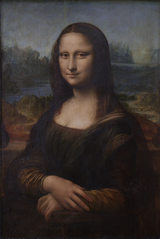
\includegraphics[width=2cm]{figs/monalisa}};
	\node[below=0 of mona, text=olivish] {{\tt monalisa.jpg}};

	% monalisa grid
	\foreach \i in {1,...,10}
	{
		\coordinate (x\i) at ($(mona.north)+(0,-2.7*\i mm)$);
		\draw[very thin, draw=black!10] (mona.west |- x\i) -- (mona.east |- x\i);

		\coordinate (y\i) at ($(mona.west)+(1.85*\i mm,0)$);
		\draw[very thin,draw=black!10] (mona.north -| y\i) -- (mona.south -| y\i);
	}

	% Tail
	\draw[cursor, <-, draw=blackish] (a4) -- +(0, 14mm)
		node[midway, right, text=blackish] (t) {Tail}
		node[TP, at end, above] (producer) {Producer thread};

	\draw[cursor, draw=olivish] (producer) to[out=180, in=0] (mona);

	% tv and monalisa output
	\node[below right=-10mm and 30mm of a4, inner sep = 0] (tv)
		{
\includegraphics[width=4cm]{figs/tv}};
	\node[below right=-5mm and 8mm of tv.west, inner sep = 0] (mona2)
		{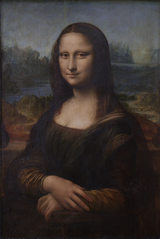
\includegraphics[width=10mm]{figs/monalisa}};

	% Head
	\draw[cursor, ->, draw=blackish]  (a2) -- +(0,-17mm)
		node[midway, right, text=blackish] (h) {Head}
		node[TC, at end, below] (consumer) {Consumer thread};
	\draw[cursor, draw=magentish, ->] (consumer) to[out=0, in=180] (tv);

	\end{tikzpicture}
	\end{center}
\end{frame}

